\begin{question}
  \hspace*{\fill} [Note Maximale: ?]\par
  \medskip
  \noindent La figure suivante représente un secteur d'un cercle de rayon $r\,cm$ et d'angle au centre $\theta$. Le périmetre du secteur est de $20\,cm$.\par
  \medskip
  \begin{center} % or flushleft or flushright
    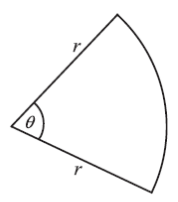
\includegraphics[scale=0.4]{figure_x3}\par
  \end{center} % or flushleft or flushright
  \begin{enumerate}[label=(\alph*)]
    \item Montrez que $\theta = \frac{20 - r}{r}$.\hspace*{\fill} [?]
    \item L'aire de ce secteur est de $25\,cm^2$. Trouvez la valeur de $r$.\hspace*{\fill} [?]
  \end{enumerate}
\end{question}
